\documentclass[12pt, a4paper, hidelinks]{article}

\usepackage[icelandic]{babel}
\usepackage[T1]{fontenc}
\usepackage[utf8]{inputenc}


\usepackage{amsmath, amssymb, amsfonts}
\usepackage{mathtools}

\usepackage[outputdir=cache]{minted}
\usemintedstyle{default}
\renewcommand{\listingscaption}{Forrit}

\usepackage{url}
\usepackage{hyperref}
\usepackage[hang, flushmargin, bottom]{footmisc}

\usepackage[svgnames]{xcolor}
\usepackage{tabularx}
\usepackage{float}
\usepackage{graphicx}
\usepackage{booktabs}
\usepackage{enumerate}
\usepackage{multirow}
\usepackage{tikz}
\usetikzlibrary{arrows}
\usepackage{pifont}
\usepackage{multicol}
\usepackage{tcolorbox}
\usepackage{forest}

\usepackage{caption}
\usepackage{subcaption}

\newcommand{\cmark}{\color{Green}\ding{51}}
\newcommand{\xmark}{\color{Red}\ding{55}}

\usepackage{times, mathptmx}
\usepackage[scaled=0.85]{beramono}

\newenvironment{code}{\captionsetup{type=listing}}{}

\usepackage{fancyhdr}
\pagestyle{fancy}
\fancyhf{}
\fancyhead[L]{Kári Hlynsson}
\fancyhead[C]{TÖL203G Heimadæmi 11}
\fancyhead[R]{\today}
\fancyfoot[C]{\thepage}

\newcommand{\doctitle}{\uppercase{Heimadæmi 11}}
\newcommand{\coursename}{Tölvunarfræði 2}
\newcommand{\coursenum}{TÖL203G}

% ——— Mengjatákn
\newcommand{\N}{\mathbb{N}}
\newcommand{\Z}{\mathbb{Z}}
\newcommand{\Q}{\mathbb{Q}}
\newcommand{\R}{\mathbb{R}}
\newcommand{\C}{\mathbb{C}}

% ——— Vigrar
\renewcommand{\u}{\mathbf{u}}
\renewcommand{\v}{\mathbf{v}}
\renewcommand{\b}{\mathbf{b}}
\newcommand{\w}{\mathbf{w}}
\newcommand{\p}{\mathbf{p}}
\newcommand{\x}{\mathbf{x}}
\newcommand{\y}{\mathbf{y}}
\newcommand{\z}{\mathbf{z}}

% Define styles for nodes in the binary tree
\tikzset{
  binarytree/.style={
    draw,
    circle,
    thick,
    minimum size=0.75cm,
    inner sep=0pt,
    font=\sffamily\small
  },
  binaryedge/.style={
    draw,
    line width=1mm,
    red
  },
  binarytree empty/.style={
    draw=none,
    fill=none
  }
}

\graphicspath{{img}}

\begin{document}
\thispagestyle{plain}
\centerline{\bfseries\Large\doctitle}
\medskip
\centerline{\large\coursenum\ \coursename}
\bigskip

\centerline{\large Kári Hlynsson\footnote{Slóð á Github kóða: \url{https://github.com/lvthnn/TOL203G/tree/master/HD11}}}
\bigskip
\centerline{Háskóli Íslands}
\medskip
\centerline{\today}

\section*{Verkefni 1}
Í þessu dæmi gerum við ráð fyrir að Bellman-Ford reikniritið vinni með leggina í hækkandi röð eftir \emph{frá}-hnúti (þ.e. hnútinum $v$ í $v \to w$).
\begin{enumerate}[(a)]
    \item Hermið reiknirit Bellman-Ford á stefnunetinu hér fyrir neðan, með upphafshnútinn 3. Sýnið stöðuna á \texttt{distTo} eftir hverja umferð.

    \item Notið hugmyndina í (a)-lið til að útbúa stefnunet með $N$ hnútum þar sem reiknirit Bellman-Ford tekur $\Theta(N^2)$ tíma. Rökstyðjið keyrslutímann.
\end{enumerate}

\begin{figure}[H]
    \centering
    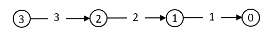
\includegraphics[width=0.75\textwidth]{HD11/pdf/img/V1.png}
    \label{fig:V1}
\end{figure}

\subsection*{Lausn}
\begin{enumerate}[(a)]
    \item Vegna þess að netið er keðja er enginn möguleiki á því að kall á \texttt{relax()} breyti gildi í \texttt{edgeTo} og \texttt{distTo} fyrir utan hina fyrstu umferð. Umferðirnar eru $|V| - 1 = 3$ talsins. Fylkið \texttt{distTo} er sett fram hér fyrir neðan eins og það leggur sig í lok hverrar umferðar.

    \begin{table}[H]
        \centering
        \caption{Staða \texttt{distTo} í upphafsstillingu}
        \begin{tabular}{lc}
            \toprule
            $v$ & \texttt{distTo[$v$]} \\
            \midrule
            3   & 0        \\
            2   & $\infty$ \\
            1   & $\infty$ \\
            0   & $\infty$ \\
            \bottomrule
        \end{tabular}
        \label{tab:my_label}
    \end{table}
    
    \begin{table}[H]
        \centering
        \caption{Staða \texttt{distTo} í umferð 1}
        \begin{tabular}{lc}
            \toprule
            $v$ & \texttt{distTo[$v$]} \\
            \midrule
            3   & 0        \\
            2   & 3         \\
            1   & 5 \\
            0   & 6 \\
            \bottomrule
        \end{tabular}
        \label{tab:my_label}
    \end{table}
    
    \begin{table}[H]
        \centering
        \caption{Staða \texttt{distTo} í umferð 2}
        \begin{tabular}{lc}
            \toprule
            $v$ & \texttt{distTo[$v$]} \\
            \midrule
            3   & 0        \\
            2   & 3         \\
            1   & 5 \\
            0   & 6 \\
            \bottomrule
        \end{tabular}
        \label{tab:my_label}
    \end{table}
    
    \begin{table}[H]
        \centering
        \caption{Staða \texttt{distTo} í umferð 3}
        \begin{tabular}{lc}
            \toprule
            $v$ & \texttt{distTo[$v$]} \\
            \midrule
            3   & 0        \\
            2   & 3         \\
            1   & 5 \\
            0   & 6 \\
            \bottomrule
        \end{tabular}
        \label{tab:my_label}
    \end{table}
    
    \item Rifjum upp að tímaflækja Bellman-Ford reikniritsins er $\Theta(|E||V|)$. Sé stefnunetið ámóta keðju eins og í (a)-lið er fjöldi leggja $|V| - 1$. Sé $|V| = N$, þá fæst $|E| = N - 1$ og því er tímaflækjan
    $\Theta\big(N(N - 1)\big)$ það er að segja $\Theta(N^2)$. Þannig er stefnunet sem uppfyllir þetta skilyrði útbúið með því að tengja hnútana í línulegri röð, eins og í dæmi (a).
\end{enumerate}

\newpage

\section*{Verkefni 2}
Segjum að við höfum stefnunet $G$ með þyngdum á leggjum. Stystu vegir hafa verið fundnir fyrir $G$ frá upphafshnúti $s$. Ef við bætum við fasta $K$ við þyngdir allra leggja $G$ þá er ekki víst að stystu vegirnir séu þeir sömu og áður. Sýnið dæmi um net þar sem þetta gildir og rökstyðjið það. Þið megið ráða þyngdum einstakra leggja og gildinu á $K$.

\end{document}
